\documentclass[notumble,combine]{leaflet}
\usepackage[dvipsnames,usenames]{color}
\usepackage{graphicx}
\usepackage{alltt}
\usepackage{url}
\usepackage{ascmac}
\usepackage{comment}
\usepackage{here}
\usepackage{wrapfig}

\makeatletter
% from leaflet.cls
\renewcommand\section{\@startsection{section}{1}{\z@}%
  {-3.5ex \@plus -.75ex}%
  {1ex} %{1.5ex}%
  {\normalfont\large\sectfont\color{NavyBlue}}}
\renewcommand\subsection{\@startsection{subsection}{2}{\z@}%
  {-2.5ex plus -.5ex}%
  {1\p@} %{1ex}%
  {\normalfont\normalsize\sectfont\color{BrickRed}}}
\makeatother

\graphicspath{{figures/}} 

\title{
	\vfill
	\includegraphics[width=\textwidth]{kbug-logo}
	\vfill
	\resizebox{\linewidth}{!}{\bf 関西*BSDユーザ会}%
	\\[\baselineskip]
        \resizebox{\linewidth}{!}{{\bf \url{http://www.kbug.gr.jp/}}}
	\vfill
        \parbox[c]{3cm}{\resizebox{3cm}{!}{\textcolor{red}{\bf{@}}}}
	\parbox[c]{4cm}{\includegraphics[width=5cm]{turret}}\\
	
\includegraphics[width=\textwidth]{osc2012-kyoto}
        \resizebox{\linewidth}{!}{{\bf \url{http://www.ospn.jp/osc2012-kyoto/}}}\\
        \resizebox{\linewidth}{!}{2012年8月3日(金),4日(土)}
}

\date{}

\begin{document}
\maketitle
\thispagestyle{empty}
\pagebreak{}
\section{関西*BSDユーザ会ってなに?}
関西 *BSD ユーザ会 (Kansai *BSD Users Group; K*BUG)とは、
BSD系OSのユーザ同士の情報交換のための{\em 場}で、1999年に設立されました。

年に数度の勉強会やイベントの参加、そして宴会を行っています。

\subsection{K*BSDの基本理念}
K*BUGの基本理念は以下のようになっています
\footnote{\url{http://www.kbug.gr.jp/charter.html}}。

\fbox{\begin{minipage}{\textwidth}
\begin{itemize}
\item 場の提供を目的とする
\item 人のケツは叩くが足は引っ張らない
\item 来るものは拒まず、猿ものは追わず
\item だれでも役員になれる。誰でも役員は止められる
\end{itemize}
\end{minipage}}

\begin{wrapfigure}[8]{r}{3cm}
\begin{center}
 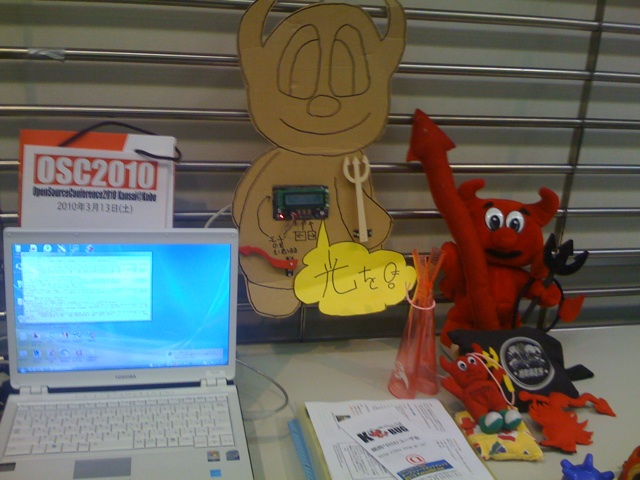
\includegraphics[width=3cm]{74251436}\\
\end{center}
\end{wrapfigure}

少し難しく感じるかもしれないですが、\textcolor{red}{BSDへの愛と情熱}があれば、
あなたが\textcolor{blue}{やりたいと思うことができる場}がK*BUGなのです。

また、メンバーは色々な技術に詳しいですし、技術に関する話も大好きなので、
あなたの疑問などもぶつけてみてください。

\section{最近の活動}
最近の活動とその内容は以下のとおりです。

もし、興味のあるテーマがあるようでしたら、是非一度遊びにきてください。

\subsection{2012年 7月29日(日)イベント@奈良高専\\\hfill (第4回研究会)}
\begin{itemize}
\item PC-BSDをはじめよう!! (インストール実習) \footnote{\url{http://qml.610t.org/FreeBSD/PCBSD.html}}
\item K*BUGをはじめよう!! \footnote{\url{http://qml.610t.org/FreeBSD/WhatIsKBUG.html}}
\item おしごとBSDを推めよう
\end{itemize}
\subsection{2012年 6月23日(土)@大阪 第3回研究会}
\subsection{2012年 4月21日(土)@京都 第2回研究会}
\begin{itemize}
\item Sony NEWSのMOをサルベージする
\item USB memstickで使うFreeBSD
\item n12iさんちのお話
\item FreeBSD portsと暮らす(2) - ports作成編\footnote{\url{http://www.slideshare.net/umq_876/making-freebsdports}}
\item FreeBSD portsと暮らす(3) - redportsを使おう\footnote{\url{http://www.slideshare.net/umq_876/using-redports}}
\item lang/squeak portの更新\footnote{\url{http://qml.610t.org/squeak4_4_7_2375.html}}
\item BSDお仕事の会のお話 (BSD-BA\footnote{\url{http://www.bsd-ba.org/}})
\end{itemize}
\subsection{2012年 2月18日(土)@大阪 第1回研究会}
\begin{itemize}
\item FreeBSD portsと暮らす(1) - github編\footnote{\url{http://www.slideshare.net/umq_876/making-freebsdports}}
\end{itemize}

\subsection{2011年12月17日(土)@大阪 \\\hfill 定期総会+第5回研究会+忘年会}
\begin{itemize}
\item USBガイガーカウンターをつなぐ+USBサウンドI/Fをつくる+USBでデジカメ制御
\item はじめてのNetBSD
\item dnssec authenicated https
\item 2011 K-OF K*BUG出展まとめとこれまでやってみて考えたこと
\end{itemize}

\subsection{2011年11月11日(金), 12日(土)@大阪 KOF 2011}
\begin{itemize}
\item OpenBSD/landiskでActive-Standby Firewall
\end{itemize}
\subsection{2011年10月15日(土)@大阪 第4回研究会}
\subsection{2011年 8月27日(土)@京都 第3回研究会}

\newpage
\subsection{2011年 7月15日(金), 16日(土)@京都 \\\hfill OSC Kansai@Kyoto 2011}
祇園祭に負けないくらい、あつい2日がそこに…

\begin{itemize}
\item NetBSD/xen (Dom0) で、 {Net, Free, Open, DragonFly}BSD (DomU)
\item makeの様子をsyslog経由で可視化する
\item {こうさく(工作, 交錯)×錯綜}する{Hack×ACK×NACK}
\end{itemize}

\begin{center}
 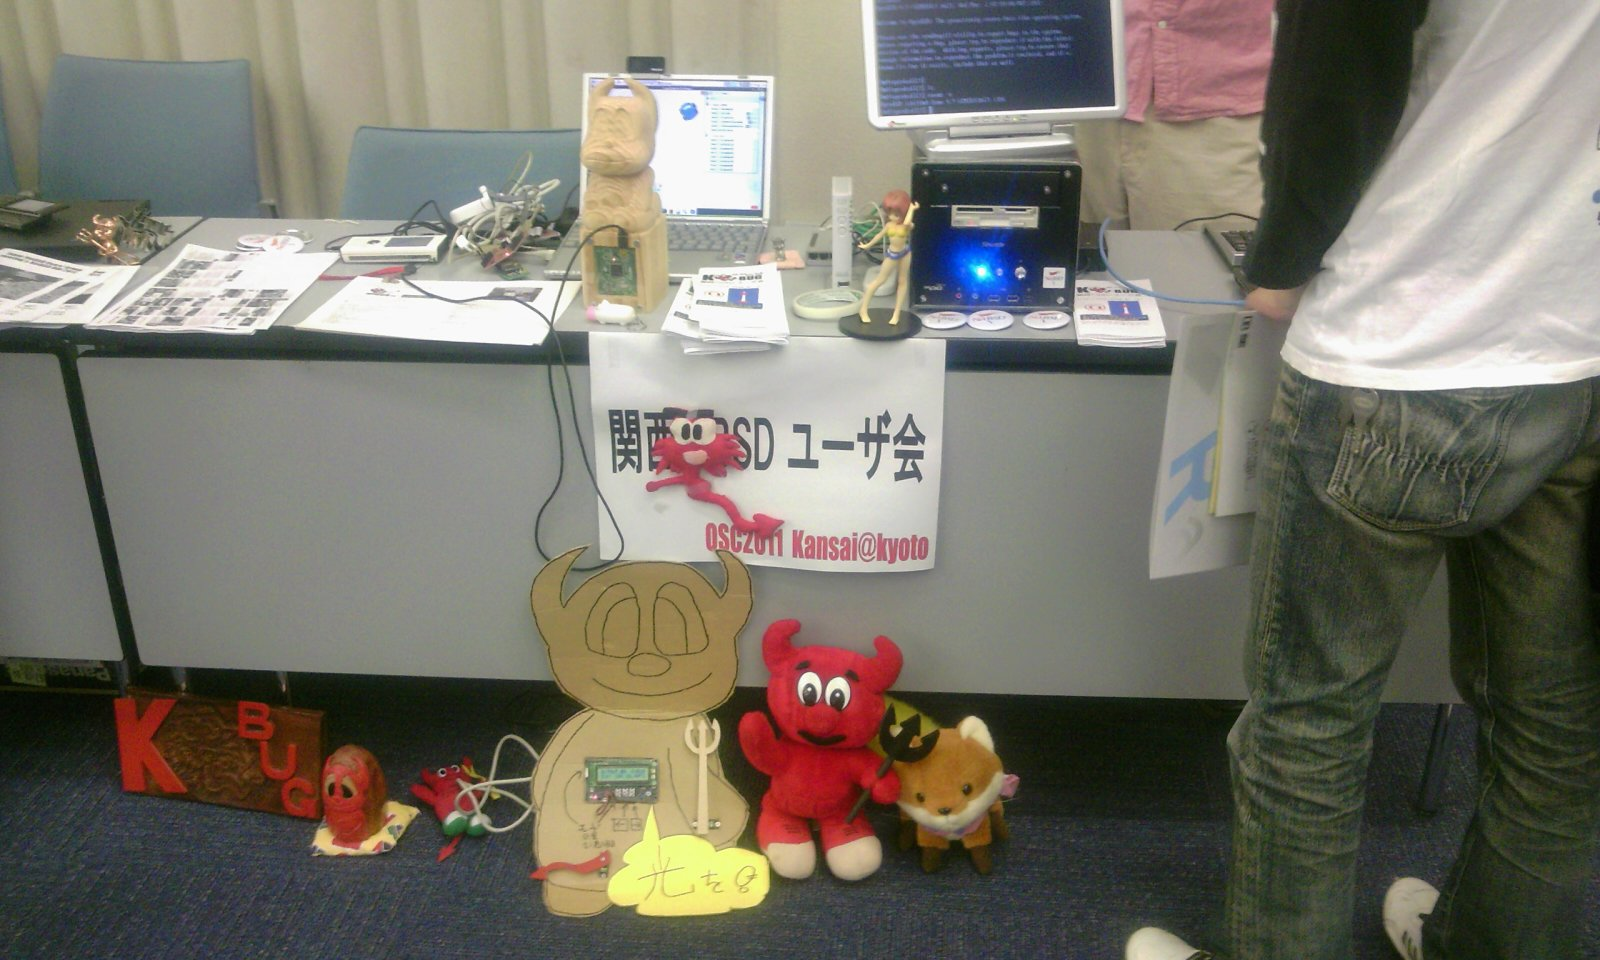
\includegraphics[width=5cm]{1310698938093}
\end{center}

\section{BSDに関する情報}
\subsection{BSD開発元リンク (日本語情報)}
\begin{itemize}
\item NetBSD情報 by JNUG\\
  \url{http://www.jp.netbsd.org/}
\item FreeBSD友の会  \url{http://www.jp.freebsd.org/}
\item OpenBSD本家  \url{http://www.openbsd.org/ja/}
\item DragonFly BSD \url{http://dragonflybsd.org/}
\end{itemize}

\subsection{ご近所BSDユーザ会リンク}
\begin{itemize}
\item JNUG(Japan NetBSD Users Group)\\
  今回もお隣でブースをさせてもらいました\\
  \url{http://www.jp.netbsd.org/ja/JP/JNUG/}
\item 名古屋*BSDユーザグループ \\ \url{http://www.nagoya.bug.gr.jp/}
\item 四国*BSDユーザ会 \\ \url{http://flathill.gr.jp/sbug/}
\end{itemize}

\newpage
\subsection{K*BUG関連}
以下のようなURLで、メンバーの活動が紹介されていますので、参考にしてください。

\begin{minipage}{\textwidth}
\begin{shadebox}
\begin{itemize}
 \item Twitter \url{http://twitter.com/610t/kbug}
 \item いしはら\hfill \url{http://www.tunagu.gr.jp/fswiki/isihara/}
 \item うえだ \\ \url{http://www.ueo.co.jp/~tueda/diary/}
 \item 西東 \url{http://d.hatena.ne.jp/tunefs/}
 \item 白井 \url{http://hp.vector.co.jp/authors/VA012337/misc/presentation.html}
 \item たけおか \url{http://www.takeoka.org/}
 \item 寺本 \url{http://d.hatena.ne.jp/mteramoto/}
 \item むとう \url{http://qml.610t.org/FreeBSD/}
 \item 野田 \url{http://d.hatena.ne.jp/akira_you/}
\end{itemize}
\end{shadebox}
\end{minipage}

\section{これからの関連イベント(予定)}
K*BUGでは、だいたい2ヶ月に1度の頻度で勉強会を行っています。
また、主に関西のイベントで、展示などを行っています。

現在、予定されているイベントは、以下のとおりです。
詳細に関しては、K*BUGのWebページをご確認ください。

\begin{itemize}
\item 2012年 8月18日(土)	第5回研究会@京都
\item 2012年10月20日(土)	第6回研究会@大阪
\item 2012年11月09(金),10(土) KOF 2012@大阪
\item 2012年12月8日(土)	第14回定期総会+第7回研究会+忘年会@大阪
\end{itemize}

\newpage
\section{K*BUG in OSC2012 Kansai@Kyoto}
\begin{itemize}
\item BSDで試すDNS64/NAT64
\item RetroBSD on PIC32マイコン\footnote{\url{http://ameblo.jp/takeoka/entry-11308169137.html}}
\item するどい*BSD
\item BSDとPhysical Computing
\end{itemize}

\subsection{NetBSDのご紹介 by JNUG}
以下のように「NetBSDのご紹介」を行いますので、ご参加ください。

\begin{itemize}
\item 日時: 2012/08/03(金) 14:00-14:45
\item 会場: アトリウム内スペース
\item 講師: 蛯原 純 (The NetBSD Project/株式会社創夢)
\item 主催:日本NetBSDユーザーグループ
\item 対象者:オペレーティングシステム/組み込み機器/ワークステーション/WZERO3/mikutterに興味がある方。
\item レベル:初級〜中級者向け
\item \url{https://www.ospn.jp/osc2012-kyoto/modules/eguide/event.php?eid=3}
\end{itemize}

NetBSDは、自由に利用可能で、BSDライセンスに基づき再配布可能な
UNIX-likeオペレーティングシステムです。
NetBSDの概要および最近の動向をご紹介します。

\begin{comment}
BSD系UNIXを取り巻く環境と、将来の展望について議論し、 BSDコミュニティ間の情報交換を行なうBOFセッションです。
4.4BSDの流れをくむFreeBSD/NetBSD/OpenBSDなど、 BSD系UNIXのユーザグループ合同で、BSD系UNIX全般を対象とした幅広いテーマで議論します。
\end{comment}

\vfill

\begin{minipage}{\textwidth}
\begin{boxnote}

\section{kbug-usersメーリングリスト}
K*BUGでは、K*BUGメンバーの情報交換や、イベントなどの情報伝達用に
kbug-usersメーリングリストを用意しています。

K*BUGメンバーは、基本的にはこのメーリングリストを読んでいることが期待
されます。

購読は以下のURLをご参照ください。

 \url{http://www.kbug.gr.jp/maillist.html}
\end{boxnote}
\end{minipage}

%\vfill

\end{document}  
